
\section*{Введение}

	\addcontentsline{toc}{section}{Введение}
	
	Довольно заметная часть звезд находятся внутри кратных или двойных системы. В двойной системе более массивная звезда эволюционирует быстрее и, в конечном счете, превращается в компактный объект, как например белый карлик, нейтронная звезда или черная дыра. Когда менее массивная звезда доходит до стадии расширения, в случае, если она находится достаточно близко к компактной звезде, ее внешние слои начинают перетекать на компактный компонент. Газ перетекает в аккреционный диск вокруг компактного компаньона, вращается, нагревается и в конце концов падает на компактную звезду. Кинетическая энергия аккрецируеммого вещества переходит в энергию излучения (при этом максимум интенсивности приходится на рентгеновский и мягкий гамма-диапазон). Изучение этого излучения может помочь понять свойства аккрецирующих объектов и механизмы генерации излучения.

	Нейтронные звезды быстро вращаются при возникновении (всё-таки звезда уменьшилась в тысячи раз, а масса только в половину), но со временем они замедляются, поскольку излучают, ускоряют заряженные частицы и теряют часть своей энергии. Скорость вращения нейтронной звезды снижается настолько, что веществу теперь ничего не препятствует падать на такую нейтронную звезду. Падая, вещество, уже будучи в состоянии плазмы, движется по линиям магнитного поля и ударяется о твёрдую поверхность тела нейтронной звезды в районе её полюсов, разогреваясь до десятков миллионов градусов. Вещество, нагретое до столь высоких температур, ярко светится в рентгеновском диапазоне. Область, в которой происходит столкновение падающего вещества с поверхностью тела нейтронной звезды, очень мала — всего около 100 метров. Это горячее пятно из-за вращения звезды периодически пропадает из вида, поэтому наблюдаются регулярные пульсации рентген-излучения. Такие объекты и называются рентгеновскими пульсарами. 	
	
	В космосе существуют тесные двойные системы, состоящие из компактного объекта (черной дыры или нейтронной звезды) и звезды-компаньона. Они могут быть источниками пульсирующего рентгеновского и мягкого гамма-излучения, которое может быть зарегистрировано различными космическими приборами (INTEGRAL, Swift/BAT, Konus-Wind и другие).
	
	Такие двойные системы играют ключевую роль в понимании процессов аккреции и выбросов с компактных объектов в присутствии сильного магнитного и гравитационного поля, поэтому их изучение может помочь понять свойства аккрецирующих объектов и механизмы генерации излучения.
	
	Суть работы заключается в анализе данных наблюдения за рентгеновскими пульсарами и 	кандидатами в черные дыры с космических аппаратов, дальнейшее определение параметров таких особенностей компактных объектов, как квазипериодические осцилляции и их эволюция со временем.
	
	Методика состоит в поиске значимых гармоник в данных с прибора и сопоставление из с известными источниками данные к которым приведены, например в статье Ларса Бильдстена <<Observation of Accreting Pulsars>> (в ней представлены характеристики аккрецирующих пульсаров на момент 1997 года). Для MAXI J1820+070 предполагается анализ квазипериодических осцилляции, регистрируемых как широкая линия в спектре мощности.
	
	Кандидат в черную дыру MAXI J1820+070 был впервые зарегистрирован 11 марта 2018 года с помощью прибора MAXI и был отождествлен с оптическим объектом ASASSN-18ey. Интенсивность источника достигла 3 Crab и её видимая звездная величина достигла значения $m_{V} = 12$ -- $13$. Столь яркое событие позволило наблюдать источник в различных диапазонах волн и различными космическими и наземными обсерваториями.  
	
	Квазипериодические колебания были в открыты в начале 80-х годах у нескольких маломассивных рентгеновских двойных. В отличие от периодического излучения, излучение этих объектов менялось в каких-то пределах: существенная часть излучения испытывала <<квазиколебания>> с <<квазипериодом>> от $\thicksim 0.1$ до $\thicksim 0.01$ Гц. Было предположено, что такие неустойчивые явления происходят при аккреции на нейтронные звезды, что хорошо согласовывалось с теоретическими моделями, но при дальнейшем изучении QPO были найдены и у кандидатов в черные дыры.
	
\section{Методика}
	
	Данные наблюдения взяты с трех приборов: Konus-Wind, INTEGRAL/ISGRI и Swift/BAT. Данные представляют соой несколько массивов чисел, означающих сколько фотонов было считано прибором за единицу времени. Каждый массив отличается друг от друга диапазоном энергий принимаемых фотонов.
	
	%Поменять определение про данные. --- done
	
	Конус --- гамма-спектрометр, установленный на космический аппарат \textit{GGS-Wind}. Конус-Винд состоит из двух одинаковых NaI(Tl) сцинтилляционных гамма-спектрометров (S1 и S2), расположенных на противоположных сторонах космического аппарата, что обеспечивает обзор всей небесной сферы. Каждый детектор состоит из кристалла NaI(Tl), который  просматривается фотоэлектронным умножителем (ФЭУ) через свинцовое стекло, нужное для снижения фонового излучения от космического аппарата. Попадая в детектор, гамма-квант передаёт часть или всю свою энергию
веществу сцинтиллятора, которая преобразуется в световую вспышку, регистрируемую ФЭУ. Заряд, собранный с анода ФЭУ, преобразуется в импульс напряжения, который усиливается и формируется для получения максимального отношения сигнал-шум, после чего амплитуда импульса измеряется аналого-цифровым преобразователем (АЦП). Схематический вид прибора и аппарата представлен на рис. \ref{img:kw1}.  \cite{Svinkin_thesis}
	
	\begin{figure}[h!]
		\centering
		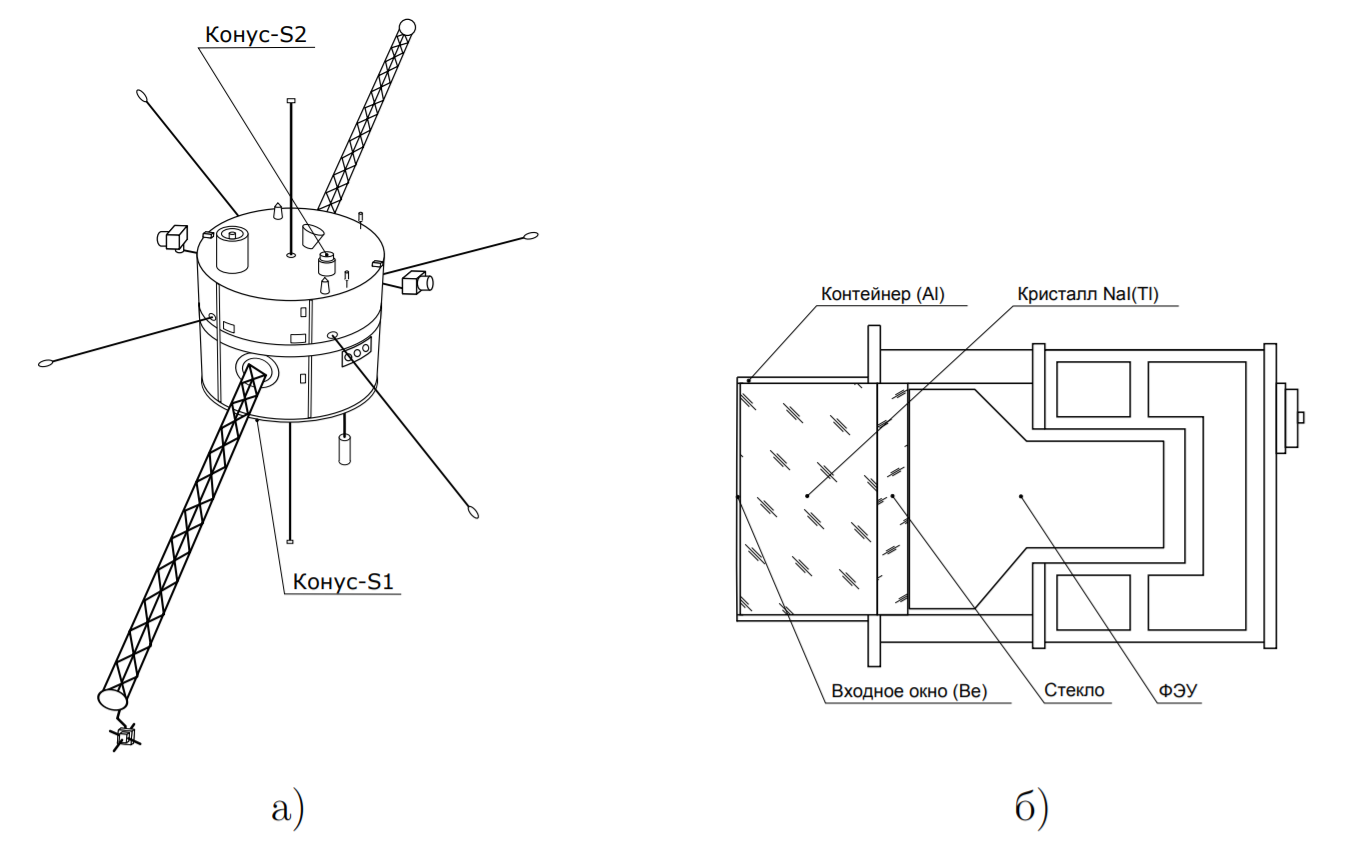
\includegraphics[width = 0.75\linewidth]{pictures/Konus-Wind.png}
		\caption{Устройство (а) спутника \textit{GGS-Wind} и (б) самого прибора}
		\label{img:kw1}
	\end{figure}
	
	BAT --- один из инструментов орбитальной обсерватории SWIFT, представляющий из себя телескоп с кодирующей маской. Кодирующая апертура является одним из способов построения изображения источника в жестком рентгеновском и мягком гамма диапазоне 
%	 (указать примерные границы диапазонов и чем они определяются физически) 
	без использования системы линз и зеркал. Метод широко применяется в гамма- и рентген-астрономии, в том числе и в INTEGRAL/ISGRI. Сигнал регистрирует массив
%	пояснить про CdZnTe-детектор
	 CdZnTe-детекторов, половина которых закрывается маской. В отличие от Konus-Wind, его поле зрения меньше и равняется $1.4$ стерадиана. На рис. \ref{img:bat1} можно увидеть схематическое представление прибора.
	 
	 CdZnTe-детекторы также, как и CdZn или NaI(Ta) являются полупроводниковыми детекторам, широко использующиеся в астрономии высоких энергий, поскольку % дописать про полупроводниковые детекторы 
	
	\begin{figure}[h!]
		\centering
			\begin{subfigure}[b]{0.49\linewidth}
			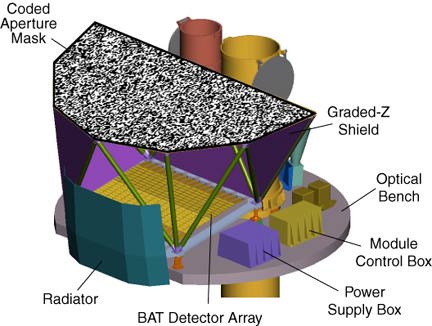
\includegraphics[width = \textwidth]{pictures/BAT.jpg}
			\caption{}
			\label{img:bat1}
		\end{subfigure}
		\begin{subfigure}[b]{0.49\linewidth}
		\centering
			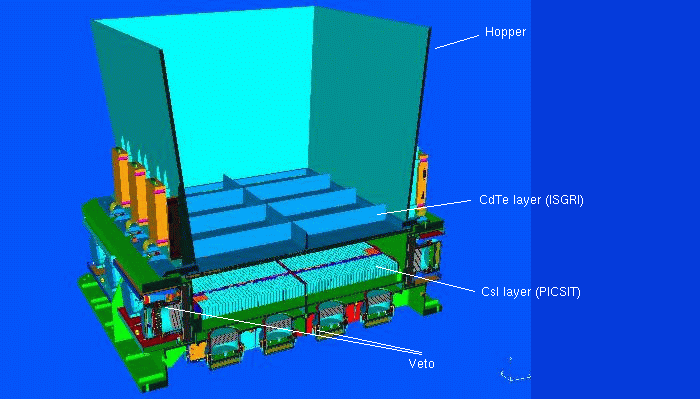
\includegraphics[width = \textwidth]{pictures/INTEGRAL.png}
			\caption{}
			\label{img:int1}
		\end{subfigure}
		\caption{Устройство прибора (a) BAT и (b) IBIS, частью которого является ISGRI}
	\end{figure}
	
	INTEGRAL аналогичен BAT, но его инструмент ISGRI импользует CdTe-детекторы и его поле зрения равно $0.26$ стерадиан. На рис. \ref{img:int1} представлено его схематическое строение. 
			 
\newpage
	
\section*{Результаты}
	
\addcontentsline{toc}{section}{Результаты}

	Преобразовение Фурье --- такое представление точкам точек, что ...

	%дописать про преобразование Фурье и спектр мощности	
	На данный момент сделана программа для анализа периодических сигналов, поиска значимых гармоник и их аппроксимация для дальнейшего нахождения пика QPO. Также сравнены данные по MAXI J1820+070, полученные с инструментов Konus-Wind, Swift/BAT, INTEGRAL/ISGRI, что можно увидеть ниже. Интересно то, что, несмотря на одинаковый спектр одинаковых фотонов у ISGRI и Konus-Wind, счет фотонов после пика у них разный. В конце работы будут получены зависимости амплитуды и частоты пульсирующей компоненты сигнала от времени для Vela-X1, GX301-2, A0535+262, SWIFT J0243.6+6124 и эволюция параметров QPO для MAXI1820+070.
	
% Описать G1 и G2.
	
	\begin{figure}[h!]
		\begin{subfigure}[b]{0.45\textwidth}
			\centering
			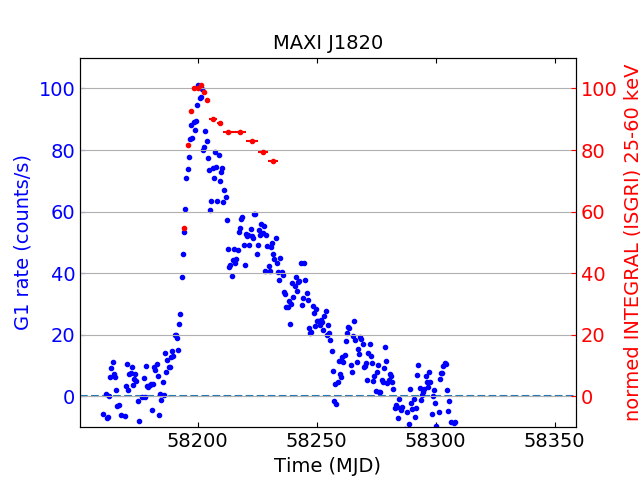
\includegraphics[width=\textwidth]{pictures/MAXIJ1820_kwG1_int.png}
			\caption{}
		\end{subfigure}
		\begin{subfigure}[b]{0.45\textwidth}
			\centering
			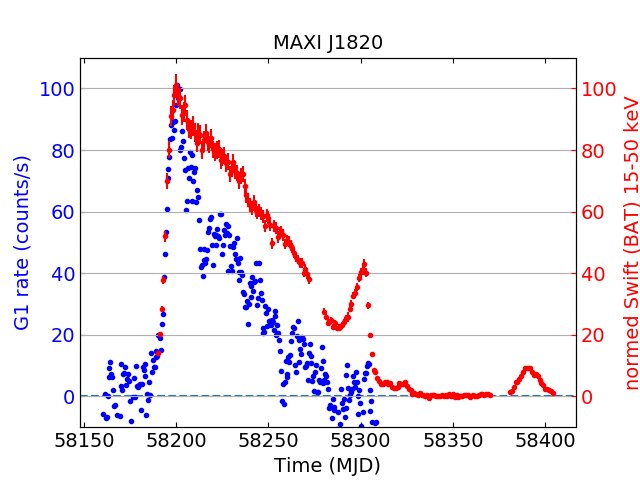
\includegraphics[width=\textwidth]{pictures/MAXIJ1820_kwG1_bat.png}
			\caption{}				
		\end{subfigure}
		\caption{Сравнение счета фотонов у Конус-Винд c (a) INTEGRAL или (b) BAT}
	\end{figure}

\newpage

\bibliography{all}	
\addcontentsline{toc}{section}{Список литературы}
